El sistema Thary fue diseñado basandose en una organizacion pipeline para el componente de prediccion y un estilo arquitectonico en capas de las cuales se distinguen tres principales:

\begin{itemize}
    \item Capa de Presentacion: Esta capa es la reponsable de funcionalidades como carga de archivos, visualizacion de resultados, registro de pedidos y demas funcionalidades relacionadas con toda la interaccion que el usuario final va a tener con el sistema.
    \item Capa de Control: Esta capa es la encargada de recibir todas las solicitudes que el usaurio le haga a la aplicacion, y devolver los resultados esperados a la capa de presentacion
    \item Capa de servicios de dominio: En esta capa se encuentra el componente de prediccion organizado como un pipeline secuencial compuesto por las diferentes etapas del sistema, en general, en esta capa se concentra toda la logica de Thary.
\end{itemize}

En cuanto a porque se decidió llevar la organizacion mediante un pipeline, esta desicion se tomo debido a que el proceso de prediccion de demanda, por su naturaleza, corresponde a un flujo secuencial de transformacion de los datos, por lo que el uso de esta estructuta facilita que se pueda separar responsabilidades de una manera mas sencilla y la trazabilidad de los resultados obtenidos. 

Por otro lado, a la hora de elegir como se manejaria la persistencia de la informacion, se opto por usar un modelo de base de datos relacional (MySQL).Esta desicion se tomo considerando la necesidad de poder contar con un historial con las corridas anteriores del sistema. Adicional a esto, la arquitectura de Thary contempla el aislamiento de los datos para cada organizacion, de manera que todas cuentan con un espcio independiente evitando que puedan acceder a informacion de otro usuario. 

\paragraph{Escenarios Arquitecturales}
% Guia: escenarios de calidad (rendimiento, disponibilidad, seguridad) que
% guian la arquitectura.
Para garantizar que Thary cuenta con una arquitectura que es capaz de responder a los atributos de calidad necesarios para un proyecto con sus caracteristicas, se plantaron los siguientes escenarios:
\begin{itemize}
    \item Escenario 1 (Confiabilidad ante datos escasos): Este escenario hace referencia a que cuando un usuario carge el historial de un producto con menos de cuatro meses de registros, Thary no debe de fallar ni excluir el producto, en su lugar, debe de utilizar un metodo de estimacion de respaldo, como la media movil. Esto le aporta valor al sistema cuando no exista suficiente informacion historica para usar un modelo mas complejo.
    \item Escenario 2 (Desempeño ante catologos extensos): Cuando se procesa un archivo con un numero alto de productos diferentes, los calculos de variables como puntos de reposicion y cantidaddes sugeridas deben de poder completarse de manera eficiente, sin que el tiempo de procesamiento se degrade de forma desproporcionada al tamaño del catalogo.
    \item Escenario 3 (Confidencialidad de la informcion): En este escenario se tiene en cuenta que Thary debe garantizar que los datos relacionados con el inventario y el historial de consumo de la organizacion, no se transmitan a ningun servicio externo del que Thary se encuentra alojado.
    \item Escenario 4 (Aislamiento entre organizaciones): Al trabajar con tantos usuarios/administradoes, lo mas probable es que en algun moemtno, al menos dos organizaciones distintar usen el sistema de manera simultane, Thary debe asegurarse que ningun tipo de dato quede expuesto ni pueda ser modificado por otra organizacion 
    \item Escenario 5 (Adaptabilidad del formato de datos): Este escenario se refiere a que cuando se cargue un archivo que pertenezca a un dominio diferente al caso de estudio principal, el cual fue salud, Thary tiene que ser capaz de reconocer y normalizar las columnas sin tener que modificar el codigo.
\end{itemize}

Estos escenarios permiten poder verificar que las desiciones arquitectonicas tomadas respondan a las necesidades que tiene el sistema, facilitando que posteriormente se pueda comprobar el funcionamiento de Thary
\paragraph{Análisis de Alternativas y Decisiones de Diseño (ADRs)}
% Guia: alternativas evaluadas y decisiones de arquitectura (ADR):
% contexto, decision, consecuencias.

Las decisiones de diseño que fueron adoptadas durante todo el desarrollo del sistema Thary y las alternativas consideradas.

\begin{itemize}
    \item Decision 1 (Persistencia basada en base de datos relacional): Debido a que el sistema va a trabajar con informacion relacionada con los usuarios y los historiales de consumo que compartan con el sistema, se tuvo que seleccionar la manera mas adecuada de almacenar dicha informacion. En una primera version de la produccion del sistema, se decidio que se utilizaran archivos estructurados independientes para cada la informacion de cada organizacion. Sin embargo, una vez se quiso mantener un registro de eventos como historial de corridas o de actividades, se migro hacia un motor de base de datos relacional MySQL.La eleccion de esta alternativa ademas de ofrecer dichas posibilidades, permite una mayor integridad de los datos y mejora la capacidad de consulta a cambio de una mayor complejidad.
    
    \item Decision 2 (Seleccion del modelo de predicccion por producto): Existen distintos productos del inventario que pueden presentar patrones de demanda diferentes entre si, teniendo esto en cuenta, al inicio del desarollo se propusieron dos alternativas, la primera era generalizar para todo el sistema el uso de un mismo modelo, y la segunda implementar tres modelos distintos. Se opto que la mejor opcion es entrenar diferentes modelos candidatos (XGBoost, regresion lineal, y media movil), comparar los resultados de los 3 y dependiendo de si el consumo es estable, esporadico o muy variable, selecccionar el que presente el menor error de prediccion, esto basandose en el calculo de el MAE (Error absoluto medio). La justificacion del porque se elijio esta metrica es que el MAE es una medida que se expresa en las mismas unidades que la demanda, lo que facilita que se pueda interpretar mas facilmente.
    
    \item Decision 3 (Validacion temporal y validacion cruzada): A la hora de validar los resultados de Thary, los cuales son conseguidos a partir de series de tiempo (historial de consumo mensual), se penso en dos propuestas, la primera se basaba en hacer una validacion cruzada aleatoria, que supone hacer una particion sin considerar el orden cronologico, mientras que la segunda se basaba en una validacion cruzada temporal de origen movil, en el que se generan varias particiones de entrenamiento y pruebas consecutivas. Se decicio optar por la segunda opcion, ya que la primera terminaria mezclando datos del futuro, lo cual se quiere evitar ya que la idea es representar un escenario real de uso del sistema, en el que no se tendrian estos datos del futuro. Es por esto que a pesar de que repetir el entrenamiento sobre varias particiones en lugar de una sola representa un mayor costo computacional, se eligio porque resulta mas representativa al desempeño real que se espera que tenga el sistema.    
\end{itemize}
        
\paragraph{Representación de la Arquitectura (Modelo C4)}
% Guia: diagramas C4: contexto, contenedores, componentes y (si aplica) codigo.

% ---------------------------------------------------------------------
% EJEMPLO DE FIGURA (borrelo y ponga la suya)
%   - guarde su imagen en la carpeta images/
%   - \includegraphics[width=...]{nombre-del-archivo}  (sin la extension)
%   - el \label debe ir DESPUES del \caption
%   - se referencia en el texto con \ref{fig:c4-contexto}
% ---------------------------------------------------------------------
\begin{figure}[H]
    \centering
    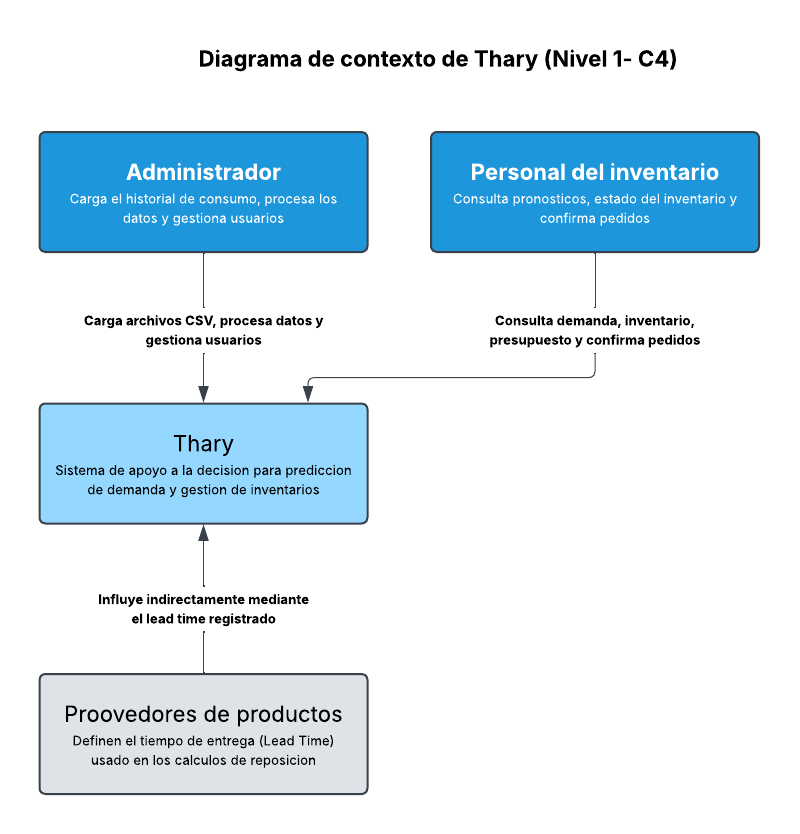
\includegraphics[width=0.7\textwidth]{templatefigures/Nivel1_Contexto}
    \caption{Diagrama de contexto del sistema (nivel 1 del modelo C4).}
    \label{fig:c4-contexto}
\end{figure}

Como se observa en la Fig. \ref{fig:c4-contexto}, el sistema interactúa con los actores identificados en la sección \ref{sec:stakeholders}.

\begin{figure}[H]
    \centering
    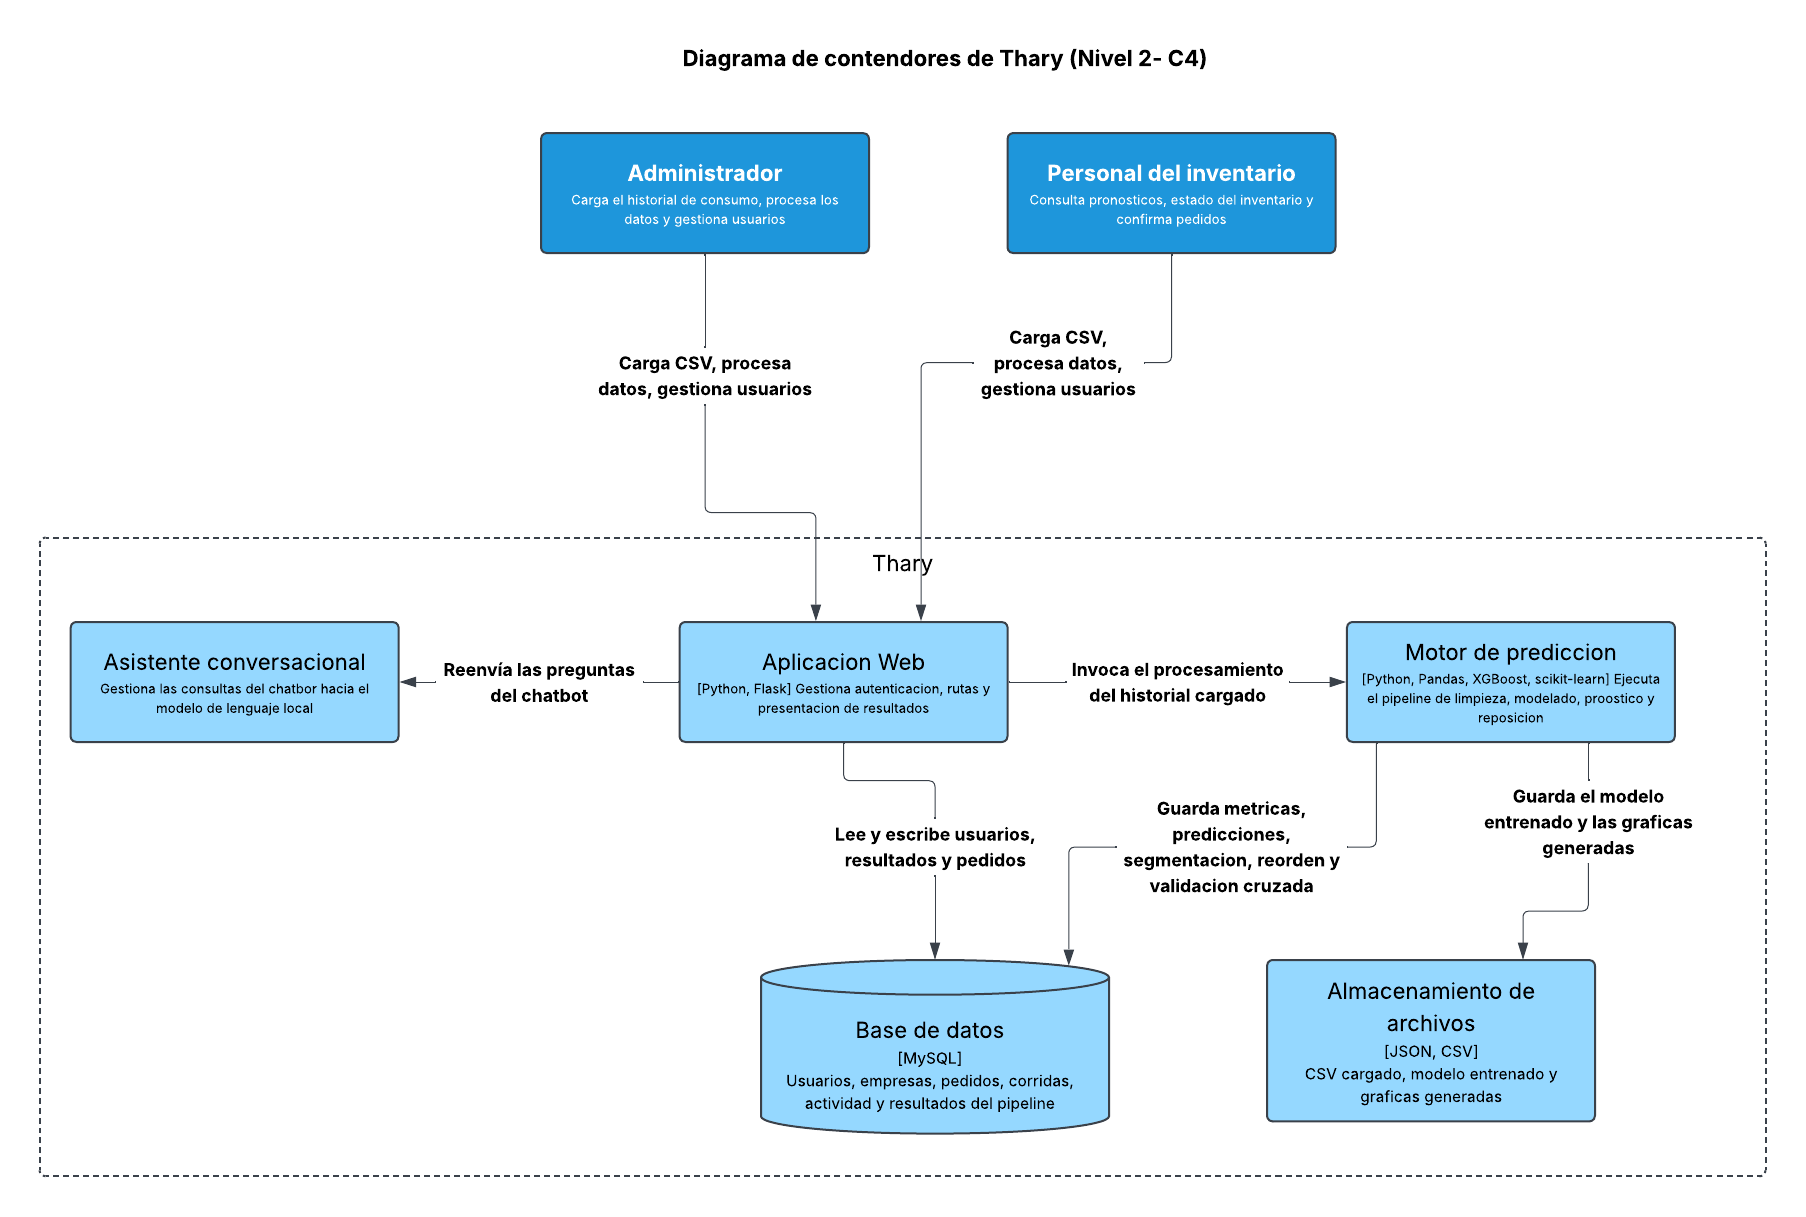
\includegraphics[width=0.7\textwidth]{templatefigures/Nivel2_Contenedores}
    \caption{Diagrama de contenedores del sistema (nivel 2 del modelo C4).}
    \label{fig:c4-contenedor}
\end{figure}

En la figura \ref{fig:c4-contenedor} se puede observar como se organizaron los contenedores del sistema Thary, factores como la aplicacion web, el motor de prediccion y la base de datos son contenedores independientes que se comunican entre si para el correcto funcionamiento del sistema. 

\begin{figure}[H]
    \centering
    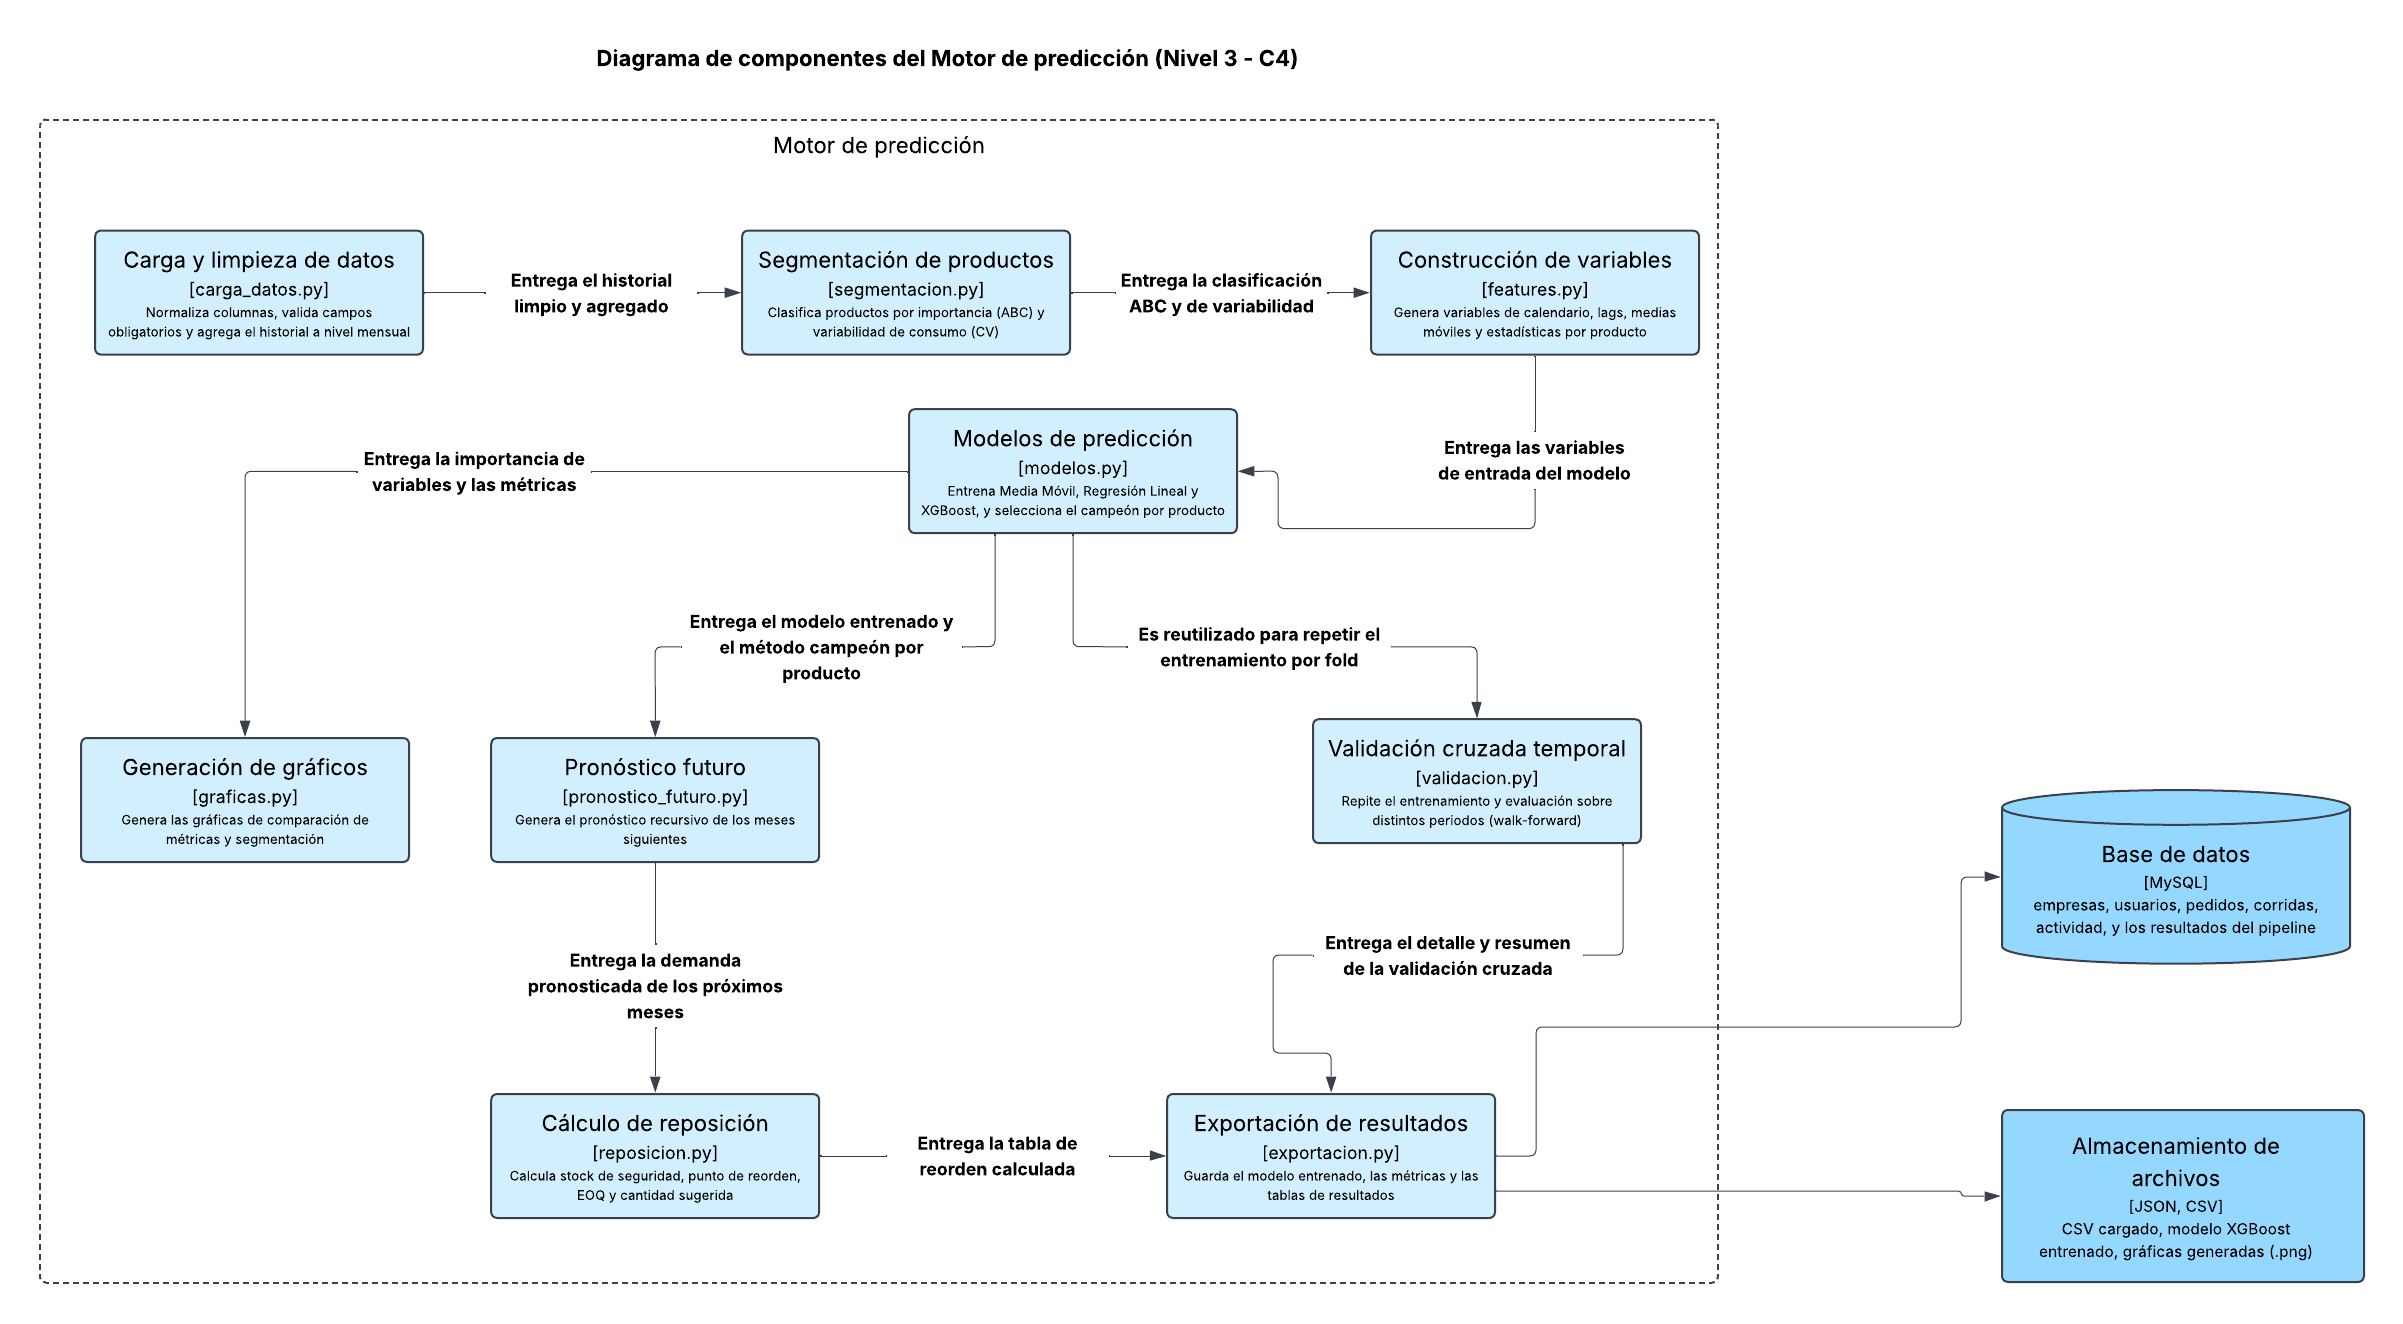
\includegraphics[width=0.7\textwidth]{templatefigures/Nivel3_Componentes}
    \caption{Diagrama de componentes del sistema (nivel 3 del modelo C4).}
    \label{fig:c4-componente}
\end{figure}

Finalmenente, el diagrama de componentes detalla a profundidad el funcionamiendo interno del motor de predicciones.
